\section{Overview}
This chapter presents the resulting findings from training and testing the recurrent neural networks, and the results from applying the predictive models to the suggested portfolio strategies. The second section presents an analysis of predictive performance when applied to small cap and large cap stock returns. Section three presents an analysis on financial results from implementing the different portfolio strategies, where small cap portfolio performance is measured before transaction costs and compared with large cap portfolio performance. Portfolio performance after transaction costs is assessed on the basis of only including costs related to broker commissions in the backtesting. An assumption with backtesting the models is that portfolio positions are re-balanced during the closing auction call, which means that there is no need for including arrival costs related to the bid-ask spread. Lending fees for short-selling and implementation shortfall is not simulated. Lastly, small cap and large cap portfolio performance is compared with the returns of a diversified small cap portfolio and a diversified large cap portfolio, which are based on all stocks included in the data sets. This gives suitable reference measures to assess whether or not recurrent neural networks can be employed to predict small cap stock returns and if they can be used as a trading tool for consistently achieving excess returns. 

\subsection{Models}
The listed models below are the selected RNNs for predicting the probability of a stock outperforming the cross-sectional median return the next day (t+1). There are a total of 12 selected models from 6 different variations of RNNs, as a result of each network being applied to small cap and large cap stocks:

\indent \newline
\begin{itemize} 
\item {\textbf{lstm1\_small/large:} This is the network which trains on all stocks simultaneously, with only one input feature of the previous 240 stock returns.}  
\item {\textbf{lstm2\_small/large} This is the network which also trains on all stocks simultaneously, but an extra LSTM-layer is included in the network structure. It trains on only one input feature, which is the previous 240 stock returns.}
\item {\textbf{lstm3\_small/large:} The third LSTM-network trains on all stocks simultaneously, but with three LSTM-layers in the network structure. It trains on only one input feature, which is the previous 240 stock returns.}
\item {\textbf{lstmi8\_small/large:} The last LSTM-variation trains on all stocks simultaneously with additional input features of the VIX, brent-crude oil price, US 10-years treasury yield, USD/NOK exchange rate, and technical indicators consisting of 50- and 200-days moving averages.}
\item {\textbf{gru1\_small/large:} This is the GRU-network which trains on all stocks simultaneously, with one input feature of the previous 240 stock returns.}
\item {\textbf{grui8\_small/large:} This is the GRU-variation which trains on all stocks simultaneously with additional input features of the VIX, brent-crude oil price, US 10-years treasury yield, USD/NOK exchange rate, and technical indicators consisting of 50- and 200-days moving averages.}
\end{itemize}   

\subsection{Hyperparameters}
\begin{table}[ht]
\centering
\resizebox{\textwidth}{!}{\begin{tabular}{l|cccccc}
\toprule
 & lstm1\_small/large & lstm2\_small/large & lstm3\_small/large & lstmi8\_small/large & gru1\_small/large & grui8\_small/large \\ \midrule
Number of layers & 1 & 2 & 3 & 1 & 1 & 1 \\
Hidden units layer 1 & 50 & 50 & 50 & 50 & 50 & 50 \\
Hidden units layer 2 & - & 50 & 50 & - & - & - \\
Hidden units layer 3 & - & - & 50 & - & - & - \\
Output neurons & 1 & 1 & 1 & 1 & 1 & 1 \\
Activation function & Sigmoid & Sigmoid & Sigmoid & Sigmoid & Sigmoid & Sigmoid \\
Optimizer & RMSProp & RMSProp & RMSProp & RMSProp & RMSProp & RMSProp \\
Training steps & 2000 & 2000 & 2000 & 2000 & 2000 & 2000 \\
Batch size & 500 & 500 & 500 & 500 & 500 & 500 \\
Learning rate & 0.005 & 0.005 & 0.005 & 0.005 & 0.005 & 0.005 \\
Dropout & 0.1 & 0.1 & 0.1 & 0.1 & 0.1 & 0.1 \\ \bottomrule
\end{tabular}}
\caption{Hyperparameters}
\end{table}
\indent \newline
Table 5.1 shows the different hyperparameters incorporated in each of the RNNs. While comparing predictive performance between small caps and large caps is the main objective, and not optimizing model performance, hyperparameters-tuning has been carried out without achieving any significant changes to predictive performance. To reduce potential differences (and sources of error) when comparing predictive performance between small cap and large cap, the different hyperparameters are kept the same for each model.   
  
\section{Predictive Performance}
\begin{table}[ht]
\centering
\resizebox{\textwidth}{!}{\begin{tabular}{l|cccccc}
\toprule
 & \textbf{lstm1\_small} & \textbf{lstm2\_small} & \textbf{lstm3\_small} & \textbf{lstmi8\_small} & \textbf{gru1\_small} & \textbf{grui8\_small} \\ \midrule
Accuracy & 0.5829 & 0.5684 & 0.5637 & 0.5694 & \textbf{0.5840} & 0.5771  \\
Precision & 0.7572 & 0.6944 & 0.6781 & 0.7661 & \textbf{0.8726} & 0.7768  \\
Recall & \textbf{0.6144} & 0.6136 & 0.6125 & 0.6009 & 0.5974 & 0.6054  \\
F1-score & 0.6784 & 0.6515 & 0.6436 & 0.6735 & \textbf{0.7093} & 0.6805  \\
Binary cross-entropy & 0.687 & 0.755 & 0.794 & 0.765 & \textbf{0.664} & 0.689  \\ \bottomrule
\end{tabular}}
\caption{Predictive performance for small cap}
\end{table}

\begin{table}[ht]
\centering
\resizebox{\textwidth}{!}{\begin{tabular}{l|cccccc}
\toprule
 & \textbf{lstm1\_large} & \textbf{lstm2\_large} & \textbf{lstm3\_large} & \textbf{lstmi8\_large} & \textbf{gru1\_large} & \textbf{grui8\_large} \\ \midrule
Accuracy & 0.5037 & \textbf{0.5089} & 0.5071 & 0.5031 & 0.5081 & 0.5042  \\
Precision & 0.5485 & 0.5410 & 0.5636 & 0.6220 & 0.6227 &  \textbf{0.6649}  \\
Recall & 0.5116 & \textbf{0.5169} & 0.5145 & 0.5100 & 0.5139 & 0.5101  \\
F1-score & 0.5294 & 0.5286 & 0.5379 & 0.5605 & 0.5631 & \textbf{0.5773}  \\
Binary cross-entropy & 0.785 & 0.910 & 0.909 & 0.893 & \textbf{0.711} & 0.733  \\ \bottomrule
\end{tabular}}
\caption{Predictive performance for large cap}
\end{table}

\indent\newline
Tables 5.2 and 5.3 highlights predictive performance for the different models when predicting returns for small cap and large stocks. Table 5.1 shows that the overall best performing model for small cap is gru1\_small, scoring highest on accuracy, precision, F1-score and cross-entropy (lowest), while the lstm1\_small has the highest score on recall. For large cap stock returns, lstm2\_large barely outperforms the other models on measures of accuracy and recall. grui8\_large scores the highest on precision and F1-score, while gru1\_large has the best binary cross entropy score. It seems implementing additional layers in the network structure does not have any significant effect on predictive performance. This can be a result of the networks needing further fine-tuning of hyperparameters, or more observations for training. The additional input features also seems to have only a minor effect on model performance, which can be a result of previous returns reflecting all factors with an influence on share price.

\indent\newline
\begin{table}[ht]
\centering
\resizebox{\textwidth}{!}{\begin{tabular}{l|cccc}
\hline
 & \textbf{gru1\_small} & \textbf{grui8\_small} & \textbf{grui8\_large} & \textbf{gru1\_large} \\ \midrule
Accuracy & \textbf{0.5840} & 0.5771 & 0.5042 & 0.5081 \\
Precision & \textbf{0.8726} & 0.7768 & 0.6649 & 0.6227 \\
Recall & 0.5974 & \textbf{0.6054} & 0.5101 & 0.5139 \\
F1-score & \textbf{0.7093} & 0.6805 & 0.5773 & 0.5631 \\
Binary cross-entropy & \textbf{0.664} & 0.689 & 0.733 & 0.711 \\ \bottomrule
\end{tabular}}
\caption{Comparison of top performing models}
\end{table}

\indent\newline
Table 5.4 illustrates the top two models for each group of stocks, based on equally weighting each performance measure. Comparing predictive performance across both group, shows that predictive models trained on small cap data outperforms models trained on large cap data on every performance measure. There are relatively big differences in all measures. The accuracy for the large cap models are just above 50\%, which is close to a random guess, while the two small cap models have accuracy measures of 58.4\% and 57.7\%, respectively. The binary cross entropy score is arguably the most important performance measure, as it accounts for how far the predicted probabilities are from the true values, and is the basis for which stocks to invest in. Also here, the small cap models outperform the large cap models with scores of 0.664 and 0.689, and 0.733 and 0.711 for the large cap models.     

\section{Portfolio Performance before Transaction Costs}
The following section presents the results from backtesting each model with a portfolio strategy consisting of only long-positions. The models instruct which five stocks to invest in each trading day, based on the predicted probability of a stock outperforming the cross-sectional median return the next day, and where all positions are weighted equally. Portfolio performance is assessed without taking into account transaction costs.    

\subsection{Small cap}
\begin{table}[ht]
\centering
\resizebox{\textwidth}{!}{\begin{tabular}{l|cccccc|c}
\toprule
Annualized & \textbf{lstm1\_small} & \textbf{lstm2\_small} & \textbf{lstm3\_small} & \textbf{lstmi8\_small} & \textbf{gru1\_small} & \textbf{grui8\_small} & {\color[HTML]{656565} \textbf{benchmark\_small}} \\ \midrule
Return & \textbf{1.1556} & 1.1023 & 0.8226 & 0.7030 & 0.6402 & 0.5194 & {\color[HTML]{656565} 0.1313} \\
Standard deviation & 0.3589 & 0.4120 & 0.3537 & 0.3768 & \textbf{0.3237} & 0.3320 & {\color[HTML]{656565} 0.1773} \\
Sharpe ratio & \textbf{3.1720} & 2.6341 & 2.2771 & 1.8202 & 1.9234 & 1.5128 & {\color[HTML]{656565} 0.6435} \\
Max drawdown & \textbf{0.2816} & 0.6022 & 0.6121 & 0.4382 & 0.5852 & 0.4265 & {\color[HTML]{656565} 0.6354} \\
VaR 5\% & \textbf{0.5653} & 0.4247 & 0.2409 & 0.0833 & 0.1075 & -0.0265 & {\color[HTML]{656565} -0.1602} \\ \bottomrule
\end{tabular}}
\caption{Small cap trading performance (long, K=5)}
\end{table}

\indent\newline
The table above shows the annualized performance metrics for each model when applied to a long-portfolio of five stocks. The portfolio termed benchmark\_small represents a diversified portfolio consisting of each small cap stock included in the data set, and is used as a benchmark measure. Analyzing the different metrics shows that the lstm1\_small network is the top-performing model with annualized returns of 115.56\%. Further, the model generates the highest Sharpe ratio, with a ratio of 3.17, as well as the best measure on value at risk. There is a 5\% probability of realizing an annualized return lower than 56.53\%, which is an exceptionally good annualized return. Taking into consideration the substantial annualized returns, a max drawdown of 28.16 percentage points indicates a moderate to low level of downside risk during the period (in addition to the VaR-measure). The lstm2\_small is the second best performing model, with an annualized return of 110.23\%. Even though this network nearly generates the same amount of annualized returns as lstm1\_small, the portfolio composition has a higher risk, illustrated by a Sharpe ratio of 2.63 and a standard deviation of 41.2\%. It also has a higher downside risk with a max drawdown of 60.22 percentage points.  

\indent\newline 
\begin{figure}[H]
\centering
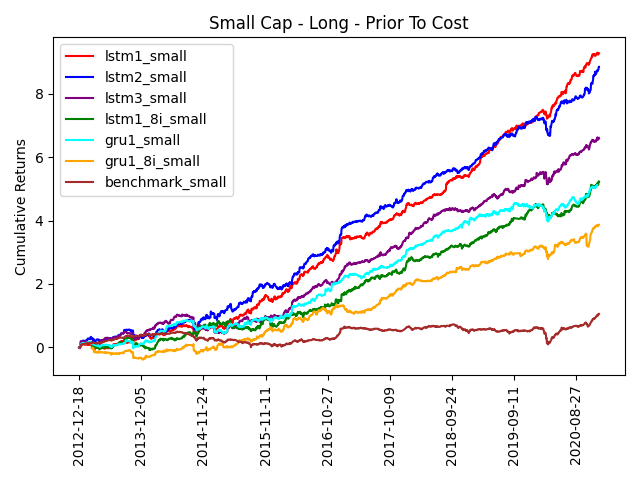
\includegraphics [scale=0.60,angle=360]{figures/cumulative_small_cap_return_no_cost.png}
\caption{Trading performance - small cap (long, K=5)}
\label{fig:smalltrading}
\end{figure}

\indent\newline 
Figure 5.1 further illustrates the findings with the two LSTM-models clearly outperforming the other models in terms of cumulative returns. The lstm1\_small generates cumulative returns of 928\%, while the worst-performing model grui8\_small generates cumulative returns of 386\%. All of the RNNs show promising results in terms of achieving excess returns, where the benchmark portfolio is outperformed with at least twice the cumulative returns, "only" generating cumulative returns of 105\%.  

\indent\newline 
An interesting part of the trading period is when the market crashed in the first half of 2020 during the breakout of the Corona-virus, and where the market cap of the Oslo Stock Exchange plummeted more than 30\% in the duration of approximately one month. While the graph illustrates each model experiencing a significant drop during the period, there is a big difference in drawdown between the top performing models. The drawdown of the lstm1\_small is relatively small considering the broad market drawdown, while the lstm2\_small experiences a much higher drawdown. This corresponds well with the lstm2\_small having higher risk, illustrated by a higher standard deviation and lower Sharpe ratio.    

\indent\newline
The analysis of predictive performance ranks gru1\_small and grui8\_small as the top-performing models for predicting small stock returns, while the analysis of portfolio performance ranks lstm1\_small and lstm2\_small as the most suitable models for achieving excess returns. A possible explanation for the differences in performance evaluation relates to the models' training process. The GRU-networks may have focused more on learning patterns within a larger number of stocks, enabling them to correctly classify a higher percentage of stocks outperforming the cross-sectional median return. The one- and two-layered LSTM may have learned patterns within a limited number of stocks that have been among the top-performing stocks during the period, enabling them to correctly predict high probabilities of the stocks that have performed well during the period. The LSTM-networks predictive performance may therefore have suffered from a higher rate of incorrect classifications, while still being able to generate higher returns.  

\subsection{Large cap}
\begin{table}[ht]
\centering
\resizebox{\textwidth}{!}{\begin{tabular}{l|cccccc|c}
\toprule
Annualized & \textbf{lstm1\_large} & \textbf{lstm2\_large} & \textbf{lstm3\_large} & \textbf{lstmi8\_large} & \textbf{gru1\_large} & \textbf{grui8\_large} & {\color[HTML]{656565} \textbf{benchmark\_large}} \\ \midrule
Return & 0.1576 & 0.1956 & 0.0805 & 0.1501 & 0.1911 & \textbf{0.2268} & {\color[HTML]{656565} 0.1539} \\
Standard deviation & 0.2733 & 0.2595 & \textbf{0.2443} & 0.2679 & 0.2616 & 0.2498 & {\color[HTML]{656565} 0.1782} \\
Sharpe ratio & 0.5135 & 0.6873 & 0.2590 & 0.4957 & 0.6648 & \textbf{0.8388} & {\color[HTML]{656565} 0.7670} \\
Max drawdown & 0.7419 & 0.8058 & \textbf{0.5564} & 0.5984 & 0.9088 & 0.8770 & {\color[HTML]{656565} 0.5535} \\
VaR 5\% & -0.2918 & -0.2311 & -0.3212 & -0.2906 & -0.2390 & \textbf{-0.1840} & {\color[HTML]{656565} -0.1391} \\ 
\bottomrule
\end{tabular}}
\caption{Large cap trading performance (long, K=5)}
\end{table}
\indent\newline 
Employing the selected RNNs to predicting large cap stock returns  results in much smaller differences between the models' portfolio performance, compared to the models employed to predicting small cap stock returns. Table 5.6 ranks grui8\_large as the best-performing model with an annualized return of 22.68\% and a Sharpe ratio of 0.84. It is also the top-performing model when assessing value at risk with a VaR of -18.4\%. On the other hand, it has one of the highest max drawdowns with a drawdown of 87.7 percentage points. The second best-performing model is lstm2\_large with an annualized return of almost 20\% and a Sharpe ratio of 0.69. It has a slightly lower max drawdown of 80 percentage points and -23\% VaR. lstm3\_large is the worst-performing RNN with annualized returns of 8\%, Sharpe ratio of 0.26, max drawdown of 55 percentage points and a VaR of -32\%. The model has the lowest fluctuation in annualized returns, illustrated by a standard deviation of 24\%.
\indent\newline 
\begin{figure}[H]
\centering
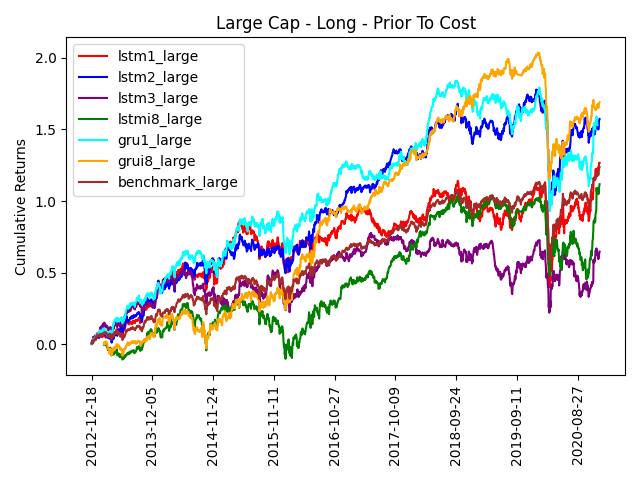
\includegraphics [scale=0.60,angle=360]{figures/cumulative_large_cap_return_no_cost.png}
\caption{Trading performance - large cap (long, K=5)}
\label{fig:largetrading}
\end{figure}
\indent\newline 
The graphical representation of cumulative returns further emphasizes the findings. Even though most of the RNNs outperform the large cap benchmark in terms of greater annualized returns, only grui8\_large is able to realize a higher Sharpe ratio than the benchmark portfolio. In other words, when adjusting for each portfolio's level of risk, the other models underperform against the benchmark. Comparing predictive performance and portfolio performance shows that the highest ranked RNNs (grui8\_large and gru1\_large) in terms of predictive performance are among the models that generates the highest annualized returns. This is more consistent than the models employed to predicting small cap stock returns.     

\subsection{Small cap vs large cap}
\begin{table}[ht]
\centering
\resizebox{\textwidth}{!}{\begin{tabular}{l|cccc|cc}
\toprule
Annualized & \textbf{lstm1\_small} & \textbf{lstm2\_small} & \textbf{grui8\_large} & \textbf{lstm2\_large} & {\color[HTML]{656565} \textbf{benchmark\_small}} & {\color[HTML]{656565} \textbf{benchmark\_large}} \\ \midrule
Return & \textbf{1.1556} & 1.1023 & 0.2268 & 0.1956 & 0.1313 & 0.1539 \\
Standard deviation & 0.3589 & 0.4120 & \textbf{0.2498} & 0.2595 & 0.1773 & 0.1782 \\
Sharpe ratio & \textbf{3.1720} & 2.6341 & 0.8388 & 0.6873 & 0.6435 & 0.7670 \\
Max drawdown & \textbf{0.2816} & 0.6022 & 0.8770 & 0.8058 & 0.6354 & 0.5535 \\
VaR 5\% & \textbf{0.5653} & 0.4247 & -0.1840 & -0.2311 & -0.1602 & -0.1391 \\ 
\bottomrule
\end{tabular}}
\caption{Comparing trading performance (long, K=5)}
\end{table}
\indent\newline 
\begin{table}[ht]
\centering
\resizebox{\textwidth}{!}{\begin{tabular}{l|cc|c}
\toprule
Annualized & \textbf{lstm1\_small} & \textbf{grui8\_large} & \textbf{Difference} \\ \midrule
Return & \textbf{1.1556} & 0.2268 & 0.9288 \\
Standard deviation & 0.3589 & \textbf{0.2498} & 0.1091 \\
Sharpe ratio & \textbf{3.1720} & 0.8388 & 2.3332 \\
Max drawdown & \textbf{0.2816} & 0.8770 & -0.5954 \\
VaR 5\% & \textbf{0.5653} & -0.1840 & 0.7493 \\
\bottomrule
\end{tabular}}
\caption{Top performing model for small and large cap (long, K=5)}
\end{table}
\indent\newline 
Comparing portfolio performance of the top models for each group of stocks shows substantial differences in annualized returns and portfolio risk. The top performing small cap model lstm1\_small generates approximately 90\ percentage points more in annualized returns compared to the best large cap model grui8\_large. The small cap model also clearly outperforms the large cap model when adjusting for risk, represented by a 2.33 higher Sharpe ratio. There are significant differences between downside risk, where the lstm1\_small has a max drawdown of 28 percentage points and a 5\% probability of realizing annualized returns below 56.53\%. The corresponding measures for grui8\_large is 87.7 percentage points and -18.4\%. The small cap models have a higher standard deviation which points to higher fluctuations in returns, but this can be a result of having a much higher rate of increase in annualized returns. 

\indent\newline 
\begin{figure}[H]
\centering
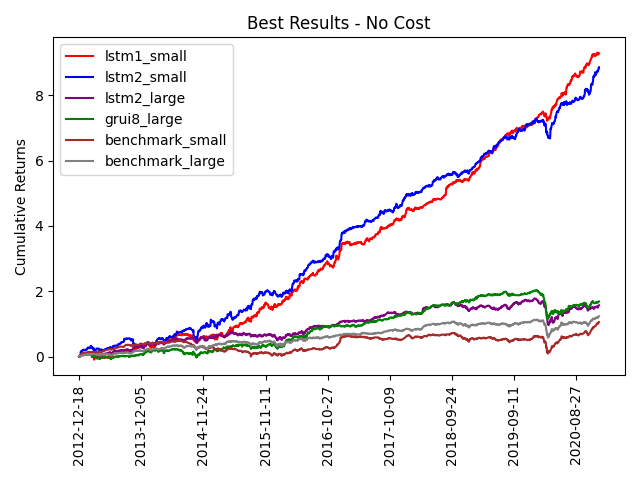
\includegraphics [scale=0.60,angle=360]{figures/cumulative_best_mix_cap_return_no_cost.png}
\caption{Small cap and large cap trading performance (long, K=5)}
\label{fig:mixtrading}
\end{figure}

\indent\newline 
Figure 5.3 shows a similar development in cumulative returns for both group of stocks during the first years of trading. In 2014 the small cap models' rate of returns starts to increase significantly more than the large cap models, while the large cap RNNs have a higher correlation with the benchmarks, resulting in a more similar development in cumulative returns throughout the period. Comparing benchmarks, shows that the small cap benchmark underperforms the large cap benchmark in the period. This should in theory be an advantage for the large cap models, as they are selecting stocks from a group with overall larger returns. A possible explanation to why the small cap models are able to outperform the large cap models, relates to the composition of the small cap group. There are often two types of companies that have a small market capitalization; young companies with expectations of experiencing a high rate of growth the coming years, and companies that are characterized by having high debt-to-equity ratios where several of them may be facing bankruptcy. This means there is a portion of small cap stocks with the potential to generate abnormal large returns, while the large cap models will not have these outperforming-stocks to choose from. When the small cap RNNs are able to differentiate between these two types of stocks, it leads to large differences in cumulative returns for the two groups of models employed to predicting stock returns. 

\indent\newline 
Having established that LSTM- and GRU-networks can be employed to predicting small cap stock returns, generate excess returns and outperform large cap stocks, the next section assess how the small cap models perform when transaction costs are included in the backtesting.

\section{Portfolio Performance after Transaction Costs}
This section implements explicit transactions costs in the form of broker commissions to evaluate the RNNs' portfolio performance in a more realistic trading environment. A fee of 3.5 basis points incurs each time a model chooses to buy or sell a stock. The commission fee is based on being a VIP-customer of Nordnet, which requires executing a minimum of 30 trades each month \cite{nordnet}. The models exceed this limit as the portfolios are re-balanced on a daily basis. 

\subsection{Small cap}
\begin{table}[ht]
\centering
\resizebox{\textwidth}{!}{\begin{tabular}{l|cccccc|c}
\toprule
Annualized & \textbf{lstm1\_small} & \textbf{lstm2\_small} & \textbf{lstm3\_small} & \textbf{lstmi8\_small} & \textbf{gru1\_small} & \textbf{grui8\_small} & {\color[HTML]{656565} \textbf{benchmark\_small}} \\ \midrule
Return & \textbf{0.7050} & 0.5595 & 0.2548 & 0.1379 & 0.1796 & -0.0535 & {\color[HTML]{656565} 0.1313} \\
Standard deviation & 0.3569 & 0.4107 & 0.3526 & 0.3760 & \textbf{0.3225} & 0.3309 & {\color[HTML]{656565} 0.1773} \\
Sharpe ratio & \textbf{1.9273} & 1.3204 & 0.6737 & 0.3208 & 0.5032 & -0.2141 & {\color[HTML]{656565} 0.6435} \\
Max drawdown & \textbf{0.3619} & 0.7544 & 0.9585 & 0.8874 & 1.0799 & 1.0187 & {\color[HTML]{656565} 0.6354} \\
VaR 5\% & \textbf{0.1180} & -0.1159 & -0.3250 & -0.4805 & -0.3510 & -0.5978 & {\color[HTML]{656565} -0.1602} \\
Total number of trades & \textbf{10,339} & 12,455 & 13,031 & 12,019 & 10,525 & 12,187 & {\color[HTML]{656565} -} \\ \bottomrule
\end{tabular}}
\caption{Small cap trading performance w/t.cost (long, K=5)}
\end{table}

\indent\newline 
Table 5.9 shows a significant (expected) drop in portfolio performance for the majority of the RNNs. The results from including transaction costs highlights the importance of models being able to identify stocks with a high probability of becoming future large cap stocks, and ultimately separate winners from losers. The lstm1\_small demonstrates a superior capability of identifying long-term winners compared to the lstm2\_small network. While the lstm2\_small model executes a total of 12,455 trades, the lstm1\_small only needs to perform 10,339 trades throughout the period. The ability of identifying winners translates into fewer trades, where winners are selected on the basis of a longer time frame, which has a large effect on portfolio performance.
\indent\newline 
\begin{figure}[H]
\centering
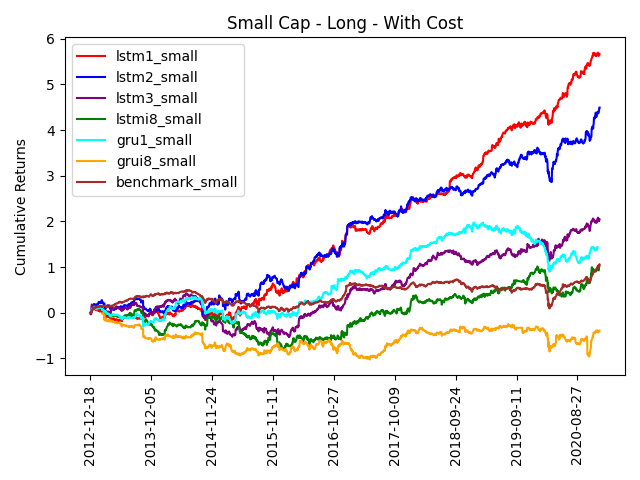
\includegraphics [scale=0.60,angle=360]{figures/cumulative_small_cap_return_with_cost.png}
\caption{Small cap trading performance w/t.cost (long, K=5)}
\label{fig:smallcost}
\end{figure}
\indent\newline 
Comparing the two top-performing models prior to transaction costs and after, highlights the impact transactions costs have on cumulative returns. Prior to transaction costs, there is only a small difference in total cumulative returns for the lstm1\_small and the lstm2\_small models (928\% vs 885\%), while after transaction costs the difference is much bigger (566\% vs 449\%). Despite the negative impact of transaction costs, every model is able to outperform the benchmark measure in terms of cumulative returns, except for the grui8\_small network. However, when adjusting for portfolio risk, only the one-layered and stacked LSTM-networks are able to outperform the benchmark, with Sharpe ratios of 1.92, 1.32 and 0.67.    

\subsection{Large cap}
\begin{table}[ht]
\centering
\resizebox{\textwidth}{!}{\begin{tabular}{l|cccccc|c}
\toprule
Annualized & \textbf{lstm1\_large} & \textbf{lstm2\_large} & \textbf{lstm3\_large} & \textbf{lstmi8\_large} & \textbf{gru1\_large} & \textbf{grui8\_large} & {\color[HTML]{656565} \textbf{benchmark\_large}} \\ \midrule
Return & -0.4671 & -0.4203 & -0.5497 & \textbf{-0.4163} & -0.4738 & -0.4706 & {\color[HTML]{656565} 0.1539} \\
Standard deviation & 0.2723 & 0.2588 & \textbf{0.2431} & 0.2676 & 0.2607 & 0.2489 & {\color[HTML]{656565} 0.1782} \\
Sharpe ratio & -1.7789 & -1.6907 & -2.3326 & \textbf{-1.6202} & -1.8837 & -1.9601 & {\color[HTML]{656565} 0.7670} \\
Max drawdown & 1.0000 & 1.0000 & 1.0000 & 1.0000 & 1.0000 & 1.0000 & {\color[HTML]{656565} 0.5535} \\
VaR 5\% & -0.9150 & \textbf{-0.8460} & -0.9496 & -0.8565 & -0.9026 & -0.8800 & {\color[HTML]{656565} -0.1391} \\
Total number of trades & 14,337 & 14,135 & 14,465 & \textbf{12,047} & 15,199 & 14,833 & {\color[HTML]{656565} -} \\ \bottomrule
\end{tabular}}
\caption{Large cap trading performance w/t.cost (long, K=5)}
\end{table}
\indent\newline 
Including transaction costs for the large cap models has an even larger negative impact on portfolio performance. None of the models are able to generate positive returns, and they are greatly outperformed by the benchmark portfolio. The least worst models are lstmi8\_large and lstm2\_large, with annualized returns of -41.63\% and -42.03\%, and Sharpe ratios of -1.62 and -1.69 respectively.  
\indent\newline 
\begin{figure}[H]
\centering
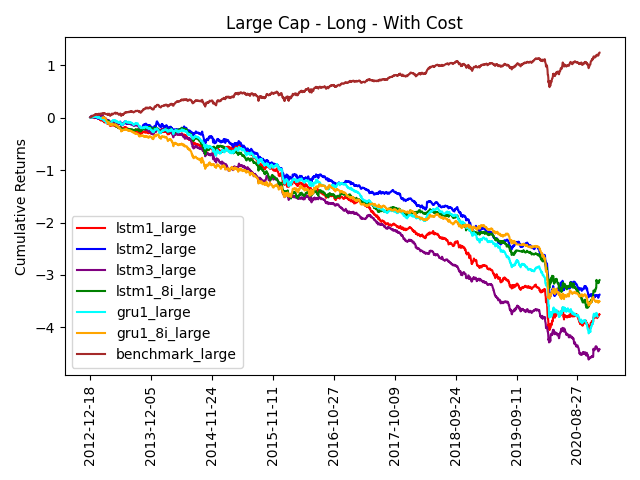
\includegraphics [scale=0.60,angle=360]{figures/cumulative_large_cap_return_with_cost.png}
\caption{Large cap trading performance w/t.cost (long, K=5)}
\label{fig:largecost}
\end{figure}
\indent\newline 
Figure 5.5 further emphasizes the findings, showing that the models' cumulative returns ranges from -309\% to -441\%, while the benchmark realizes cumulative returns of 123\%. In theory, it is not possible to generate negative returns below 100\% since the portfolio strategy consists of only being long and not short. However, the graph illustrates the resulting outcome if one were to keep adding investing capital to the portfolio throughout the period.    

\subsection{Small cap vs large cap}
\begin{table}[ht]
\centering
\resizebox{\textwidth}{!}{\begin{tabular}{l|cccc|cc}
\toprule
Annualized & \textbf{lstm1\_small} & \textbf{lstm2\_small} & \textbf{lstmi8\_large} & \textbf{lstm2\_large} & {\color[HTML]{656565} benchmark\_small} & {\color[HTML]{656565} benchmark\_large} \\ \midrule
Return & \textbf{0.7050} & 0.5595 & -0.4163 & -0.4203 & {\color[HTML]{656565} 0.1313} & {\color[HTML]{656565} 0.1539} \\
Standard deviation & 0.3569 & 0.4107 & 0.2676 & \textbf{0.2588} & {\color[HTML]{656565} 0.1773} & {\color[HTML]{656565} 0.1782} \\
Sharpe ratio & \textbf{1.9273} & 1.3204 & -1.6202 & -1.6907 & {\color[HTML]{656565} 0.6435} & {\color[HTML]{656565} 0.7670} \\
Max drawdown & \textbf{0.3619} & 0.7544 & 1.0000 & 1.0000 & {\color[HTML]{656565} 0.6354} & {\color[HTML]{656565} 0.5535} \\
VaR 5\% & \textbf{0.1180} & -0.1159 & -0.8565 & -0.8460 & {\color[HTML]{656565} -0.1602} & {\color[HTML]{656565} -0.1391} \\
Total number of trades & \textbf{10,339} & 12,455 & 12,047 & 14,135 & {\color[HTML]{656565} -} & {\color[HTML]{656565} -} \\ \bottomrule
\end{tabular}}
\caption{Comparison of trading performance w/t.costs (long, K=5)}
\end{table}

\indent\newline
\begin{table}[ht]
\centering
\resizebox{\textwidth}{!}{\begin{tabular}{l|cc|c}
\toprule
Annualized & \textbf{lstm1\_small} & \textbf{lstmi8\_large} & \textbf{Difference} \\ \midrule
Return & \textbf{0.7050} & -0.4163 & 1.1213 \\
Standard deviation & 0.3569 & \textbf{0.2676} & 0.0893 \\
Sharpe ratio & \textbf{1.9273} & -1.6202 & 3.5475 \\
Max drawdown & \textbf{0.3619} & 1.0000 & -0.6381 \\
VaR 5\% & \textbf{0.1180} & -0.8565 & 0.9745 \\
Total number of trades & \textbf{10,339} & 12,047 & -1,708 \\ \bottomrule
\end{tabular}}
\caption{Comparison of top models w/t.costs (long, K=5)}
\end{table}
\indent\newline
The tables above highlights how the small cap RNNs outperform the large cap models. Including explicit transaction costs further emphasize the vast differences in portfolio performance choosing to trade small cap stocks as apposed to large cap stocks. It is clear that employing RNNs to predict large stock returns is not a profitable trading strategy, where an investor would probably change his/hers investing strategy, rather than keep adding funds to an unsuccessful portfolio. The top-performing large cap models are able to outperform the benchmark without taking into consideration transaction costs, but when these are included they suffer from the high trading frequency.       
\indent\newline 
\begin{figure}[H]
\centering
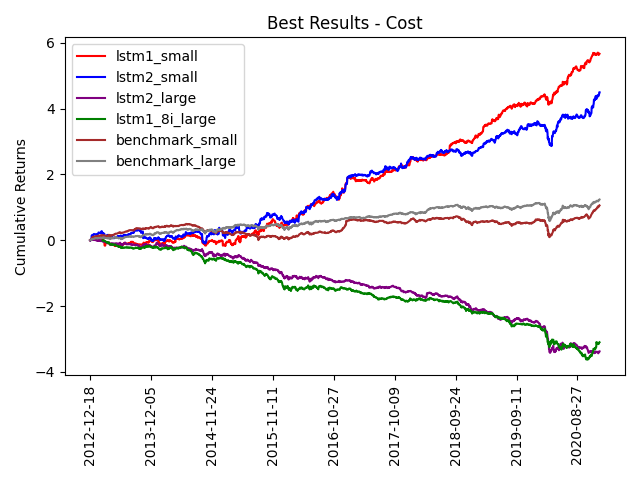
\includegraphics [scale=0.60,angle=360]{figures/cumulative_best_mix_cap_return_cost.png}
\caption{Comparison of trading performance w/t.cost (long, K=5)}
\label{fig:mixcost}
\end{figure} 
\indent\newline 
Figure 5.6 illustrates the superior performance of the small cap models. The small cap RNNs generate cumulative returns of 566\% and 449\%, while the large cap RNNs generate negative cumulative returns of 309\% and 337\%. When comparing the best-performing model for each group (lstm1\_small and lstmi8\_large) the small cap model outperforms the large cap model in terms of managing to achieve a 112 percentage points higher annualized return and a 3.54 higher Sharpe ratio. The lstm1\_small model also outperform the benchmarks, with a 1.28 higher Sharpe ratio than the benchmark\_small, and a 1.16 higher Sharpe ratio than the benchmark\_large. 

\indent\newline 
The resulting findings in this section suggest RNNs can be employed to predicting small cap stock returns for a long portfolio consisting of 5 stocks, re-balanced on a daily basis, and generate significant excess returns compared to large cap stocks. Evidence points towards the models having the ability to take advantage of the small cap stocks'  high volatility and fluctuation in share price as apposed to the lower volatility in large cap stocks.    

\indent\newline 
In the following sections, the models are tested with two additional portfolio strategies, namely a 50/50 long-short portfolio and a short-only portfolio.

\section{Additional Trading Strategies}
\subsection{Long-short 50/50 before transaction cost}
The long-short portfolio strategy consists of going long two stocks and going short two stocks, giving a total of four positions in the portfolio. As with the former strategy the portfolio is re-balanced each day, where long positions are based on the two highest predicted probabilities of a stock outperforming the cross-sectional median return, while short positions are based on the two lowest predicted probabilities.
\indent\newline 
\begin{table}[ht]
\centering
\resizebox{\textwidth}{!}{\begin{tabular}{l|cccccc|c}
\toprule
Annualized & \textbf{lstm1\_small} & \textbf{lstm2\_small} & \textbf{lstm3\_small} & \textbf{lstmi8\_small} & \textbf{gru1\_small} & \textbf{grui8\_small} & {\color[HTML]{656565} \textbf{benchmark\_small}} \\ \midrule
Return & \textbf{2.6358} & 2.0698 & 1.4935 & 1.1650 & 0.7671 & 0.3508 & {\color[HTML]{656565} 0.1313} \\
Standard deviation & 0.9795 & 1.0144 & 0.8187 & 0.9863 & \textbf{0.8777} & 1.4605 & {\color[HTML]{656565} 0.1773} \\
Sharpe ratio & \textbf{2.6732} & 2.0233 & 1.8030 & 1.1636 & 0.8543 & 0.2283 & {\color[HTML]{656565} 0.6435} \\
Max drawdown & \textbf{1.0132} & 1.0794 & 1.1876 & 1.6607 & 1.6244 & 3.5733 & {\color[HTML]{656565} 0.6354} \\
VaR 5\% & \textbf{1.0246} & 0.4012 & 0.1467 & -0.4573 & -0.6766 & -2.051 & {\color[HTML]{656565} -0.1602} \\ \bottomrule
\end{tabular}}
\caption{50/50 long-short small cap (2K, K=2)}
\end{table}
\indent\newline 
The lstm1\_small is the best-performing model, producing annualized returns of 263\% and a Sharpe ratio of 2.67. The annualized standard deviation is 97\% and there is a 5\% probability of realizing a return lower than 102\% (VaR). The worst-performing model is grui8\_small, with annualized returns of 35\% and a Sharpe ratio of 0.22. The big drop in returns for grui8\_small during the end of 2016 would require investing additional capital to the portfolio.  
\indent\newline 
\begin{figure}[H]
\centering
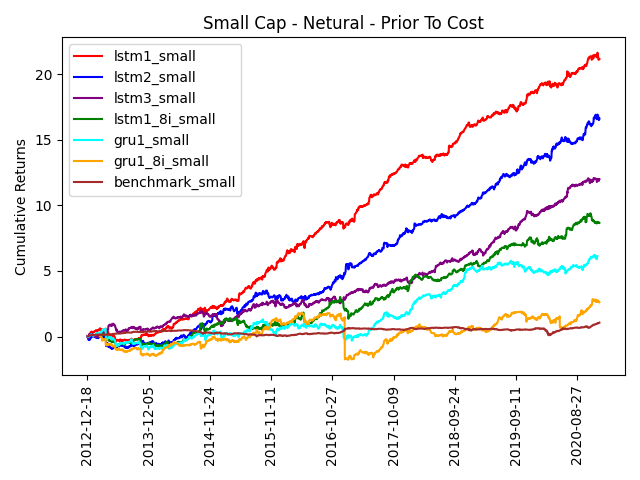
\includegraphics [scale=0.60,angle=360]{figures/cumulative_small_cap_return_no_cost_n.png}
\caption{Small cap trading performance 50/50 (2K, K=2)}
\label{fig:5050small}
\end{figure} 
\indent\newline 
The figure above displays each model realizing a higher cumulative return than the benchmark portfolio. All models outperform the benchmark in terms of having a higher Sharpe ratio, except for grui8\_small. 

\indent\newline 
\begin{table}[ht]
\centering
\resizebox{\textwidth}{!}{\begin{tabular}{l|cccccc|c}
\toprule
Annualized & \textbf{lstm1\_large} & \textbf{lstm2\_large} & \textbf{lstm3\_large} & \textbf{lstmi8\_large} & \textbf{gru1\_large} & \textbf{grui8\_large} & {\color[HTML]{656565} \textbf{benchmark\_large}} \\ \midrule
Return & -0.0884 & \textbf{0.2158} & -0.0514 & -0.1092 & -0.0762 & 0.1161 & {\color[HTML]{656565} 0.1539} \\
Standard deviation & 0.4402 & 0.3969 & \textbf{0.3795} & 0.4273 & 0.4983 & 0.3838 & {\color[HTML]{656565} 0.1782} \\
Sharpe ratio & -0.2401 & \textbf{0.5000} & -0.1809 & -0.2961 & -0.1876 & 0.2574 & {\color[HTML]{656565} 0.7670} \\
Max drawdown & 1.4138 & 1.2324 & 1.3844 & 1.3780 & 2.6298 & \textbf{0.8178} & {\color[HTML]{656565} 0.5535} \\
VaR 5\% & -0.8125 & \textbf{-0.4371} & -0.6757 & -0.8122 & -0.8959 & -0.5153 & {\color[HTML]{656565} -0.1391} \\ \bottomrule
\end{tabular}}
\caption{50/50 long-short large cap (2K, K=2)}
\end{table}
\indent\newline 
The top-performing model for the group of large cap stocks is lstm2\_large with annualized returns of 21.58\% and a Sharpe ratio of 0.50. The model has a lot more downside risk compared to the lstm1\_small represented by a 5\% probability of realizing a return lower than -43.71\%. lstmi8\_large is the worst-performing model with annualized returns of -10.92\% and a Sharpe ratio of -0.29.    
\indent\newline 
\begin{figure}[H]
\centering
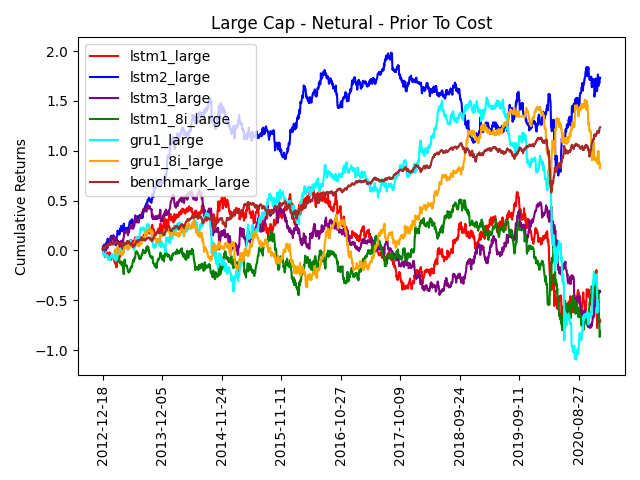
\includegraphics [scale=0.60,angle=360]{figures/cumulative_large_cap_return_no_cost_n.png}
\caption{Large cap trading performance 50/50 (2K, K=2)}
\label{fig:5050large}
\end{figure} 
\indent\newline 
The lstm2\_large is the only RNN which generates higher cumulative returns than the benchmark, but in terms of risk-adjusted returns (Sharpe ratio) none of the models are able to outperform the benchmark. Both of the GRU-networks generate higher cumulative returns than the benchmark during certain times of the trading period, but performance decline towards the end of the period.   

\indent\newline 
\begin{table}[ht]
\centering
\resizebox{\textwidth}{!}{\begin{tabular}{l|cc|c}
\toprule
Annualized & \textbf{lstm1\_small} & \textbf{lstm2\_large} & \textbf{Difference} \\ \midrule
Return & \textbf{2.6358} & 0.2158 & 2.4200 \\
Standard deviation & 0.9795 & \textbf{0.3969} & 0.5826 \\
Sharpe ratio & \textbf{2.6732} & 0.5000 & 2.1732 \\
Max drawdown & \textbf{1.0132} & 1.2324 & -0.2192 \\
VaR 5\% & \textbf{1.0246} & -0.4371 & 1.4617 \\ \bottomrule
\end{tabular}}
\caption{50/50 long-short comparison of top models (2K, K=2)}
\end{table}
\indent\newline 
A comparison of the top RNNs from each group of stocks shows extremely large differences in portfolio performance. The small cap LSTM-network generates 242 percentage points higher annualized returns and a 2.17 higher Sharpe ratio. There is also substantially less downside risk in the small cap portfolio, illustrated by a VaR of 102\% compared to a VaR of -43\%.

\indent\newline 
\begin{figure}[H]
\centering
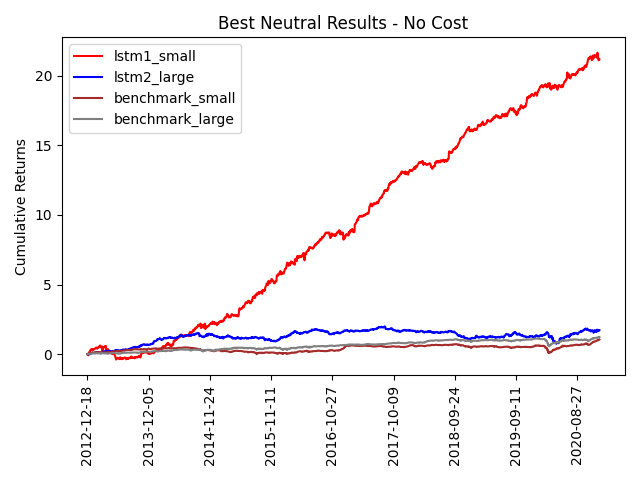
\includegraphics [scale=0.60,angle=360]{figures/cumulative_best_neutral_mix_return_no_cost.png}
\caption{Comparison of trading performance 50/50 long-short (2K, K=2)}
\label{fig:mix50}
\end{figure}

\subsection{Long-short 50/50 after transaction cost}
This section implements broker commission in order to simulate a more realistic trading environment. Fees for lending shares intended for short selling is not included in the backtesting. 
\indent\newline 
\begin{table}[ht]
\centering
\resizebox{\textwidth}{!}{\begin{tabular}{l|cccccc|c}
\toprule
Annualized & \textbf{lstm1\_small} & \textbf{lstm2\_small} & \textbf{lstm3\_small} & \textbf{lstmi8\_small} & \textbf{gru1\_small} & \textbf{grui8\_small} & {\color[HTML]{656565} \textbf{benchmark\_small}} \\ \midrule
Return & \textbf{2.1462} & 1.5309 & 0.9342 & 0.6613 & 0.2481 & -0.2203 & {\color[HTML]{656565} 0.1313} \\
Standard deviation & 0.9781 & 1.0131 & \textbf{0.8177} & 0.9855 & 0.8765 & 1.4598 & {\color[HTML]{656565} 0.1773} \\
Sharpe ratio & \textbf{2.1764} & 1.4940 & 1.1213 & 0.6534 & 0.2633 & -0.1627 & {\color[HTML]{656565} 0.6435} \\
Max drawdown & \textbf{1.1842} & 1.2057 & 1.3346 & 1.7118 & 2.6704 & 4.050 & {\color[HTML]{656565} 0.6354} \\
VaR 5\% & \textbf{0.5372} & -0.1355 & -0.4108 & -0.9597 & -1.1936 & -2.6216 & {\color[HTML]{656565} -0.1602} \\
Total number of trades & 11,236 & 12,366 & 12,836 & \textbf{10,714} & 11,864 & 12,148 & {\color[HTML]{656565} -} \\ \bottomrule
\end{tabular}}
\caption{50/50 long-short small cap w/t.cost (2K, K=2)}
\end{table}
\indent\newline 
Evaluating portfolio performance after including transaction costs shows that the lstm1\_small is the best performing model with annualized returns of 214\% and an annualized Sharpe ratio of 2.17. This means the costs related to broker commissions reduce the annualized returns with approximately 50 percentage points and the Sharpe ratio with 0.5. 
\indent\newline 
\begin{figure}[H]
\centering
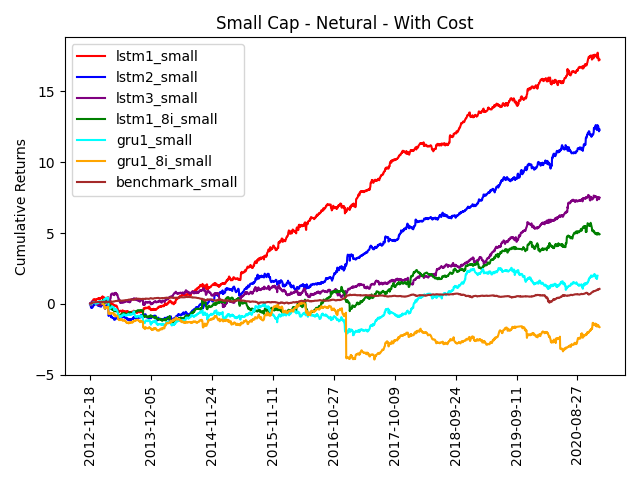
\includegraphics [scale=0.60,angle=360]{figures/cumulative_small_cap_return_with_cost_n.png}
\caption{Small cap trading performance w/t.cost 50/50 (2K, K=2)}
\label{fig:5050smallc}
\end{figure} 
\indent\newline 
All of the RNNs outperform the benchmark in terms of excess returns, except for grui8\_small. The GRU-network experiences a large drop in returns at the end of 2016, which it never recovers from. The two GRU-networks are the only models that are not able to outperform the benchmark when looking at Sharpe ratio.

\indent\newline 
\begin{table}[ht]
\centering
\resizebox{\textwidth}{!}{\begin{tabular}{l|cccccc|c}
\toprule
Annualized & \textbf{lstm1\_large} & \textbf{lstm2\_large} & \textbf{lstm3\_large} & \textbf{lstmi8\_large} & \textbf{gru1\_large} & \textbf{grui8\_large} & {\color[HTML]{656565} \textbf{benchmark\_large}} \\ \midrule
Return & -0.6427 & \textbf{-0.3538} & -0.6300 & -0.6250 & -0.6588 & -0.5042 & {\color[HTML]{656565} 0.1539} \\
Standard deviation & 0.4390 & 0.3965 & \textbf{0.3784} & 0.4266 & 0.4972 & 0.3836 & {\color[HTML]{656565} 0.1782} \\
Sharpe ratio & -1.5033 & \textbf{-0.9357} & -1.7107 & -1.5056 & -1.3597 & -1.3595 & {\color[HTML]{656565} 0.7670} \\
Max drawdown & 1.0000 & 1.0000 & 1.0000 & 1.0000 & 1.0000 & 1.0000 & {\color[HTML]{656565} 0.5535} \\
VaR 5\% & -1.3650 & \textbf{-1.0061} & -1.2525 & -1.3268 & -1.4767 & -1.1352 & {\color[HTML]{656565} -0.1391} \\
Total number of trades & 12,722 & 13,072 & 13,280 & \textbf{10,970} & 13,318 & 13,194 & {\color[HTML]{656565} -} \\ \bottomrule
\end{tabular}}
\caption{50/50 long-short large cap w/t.cost (2K, K=2)}
\end{table}
\indent\newline 
Assessing the large cap models after implementing broker commissions shows all of the models underperforming the benchmark. The lstm2\_large network is the least-worst performing model with annualized returns of -35\% and a Sharpe ratio of -0.93. The model with the lowest Sharpe ratio is lstm3\_large with a ratio of -1.71, while the model with lowest annualized returns is gru1\_large with returns of -65\%.  
\indent\newline 
\begin{figure}[H]
\centering
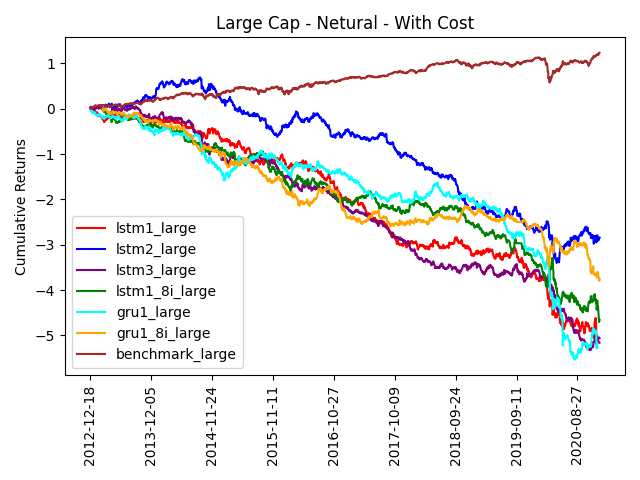
\includegraphics [scale=0.60,angle=360]{figures/cumulative_large_cap_return_with_cost_n.png}
\caption{Large cap trading performance w/t.cost 50/50 (2K, K=2)}
\label{fig:5050largec}
\end{figure} 
\indent\newline 
Figure 5.11 illustrates how all of the RNNs underperform the benchmark. The lstm2\_large outperforms the benchmark during a short period between 2013 and 2014, but quickly starts to decline after this period, ending with cumulative returns of -284\%.
\indent\newline 
\begin{table}[ht]
\centering
\resizebox{\textwidth}{!}{\begin{tabular}{l|cc|c}
\toprule
Annualized & \textbf{lstm1\_small} & \textbf{lstm2\_large} & \textbf{Difference} \\ \midrule
Return & \textbf{2.1462} & -0.3538 & 2.5000 \\
Standard deviation & 0.9781 & \textbf{0.3965} & 0.5816 \\
Sharpe ratio & \textbf{2.1764} & -0.9357 & 3.1121 \\
Max drawdown & \textbf{1.1842} & 4.0943 (1.00) & -2.9101 \\
VaR 5\% & \textbf{0.5372} & -1.0061 & 1.5433 \\
Total number of trades & \textbf{11,236} & 13,072 & -1,836 \\ \bottomrule
\end{tabular}}
\caption{Comparison top models 50/50 long w/t.cost (2K, K=2)}
\end{table}
\indent\newline 
Analyzing the top-performing model from each group of stocks highlights the massive differences in portfolio performance. The lstm1\_small RNN outperforms the lstm2\_large network in terms of generating 250 percentage points in excess annualized returns. When adjusting for risk, the large cap model is outperformed with a 3.11 higher Sharpe ratio. There is also considerably less downside risk, represented by a VaR of 53\% and -100\%. The small cap network also performs 1,836 trades less than the large cap model.  

\indent\newline 
\begin{figure}[H]
\centering
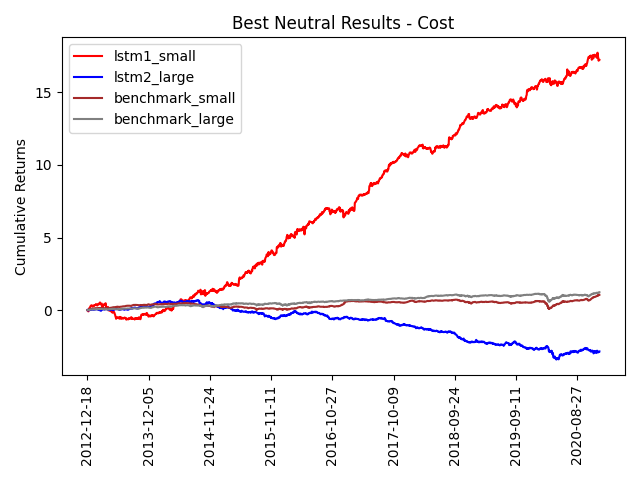
\includegraphics [scale=0.60,angle=360]{figures/cumulative_best_neutral_mix_return_cost.png}
\caption{Comparison of trading performance 50/50 long-short w/t.cost (2K, K=2)}
\label{fig:mix50c}
\end{figure}
\indent\newline 
The resulting findings suggest that the small cap models have an advantage by being able to choose from a group of stocks that have more extreme movements in returns. As discussed in section 5.3.3, when the small cap models learns the patterns and learns to differentiate between stocks that have a high probability of becoming short/long-term winners and short/long-term losers, they manage to capitalize on these extreme movements. The large cap models have less stocks to choose from with extreme movements in returns, which greatly affects performance when using a strategy that requires a high frequency of trading.

\subsection{Short-only before transaction costs}
This portfolio strategy consists of short-selling the five bottom ranked stocks, which is based on the models predicted probability of a stock outperforming the cross-sectional median return. The portfolio is re-balanced on a daily basis. The strategy does not account for potential complications regarding whether or not a stock is possible to short. 
\indent\newline     
\begin{table}[ht]
\centering
\resizebox{\textwidth}{!}{\begin{tabular}{l|cccccc|c}
\toprule
Annualized & \textbf{lstm1\_small} & \textbf{lstm2\_small} & \textbf{lstm3\_small} & \textbf{lstmi8\_small} & \textbf{gru1\_small} & \textbf{grui8\_small} & {\color[HTML]{656565} \textbf{benchmark\_small}} \\ \midrule
Return & 0.4804 & \textbf{0.4840} & 0.0641 & 0.2867 & 0.1453 & 0.3144 & {\color[HTML]{656565} 0.1313} \\
Standard deviation & 0.6716 & 0.4700 & 0.6196 & \textbf{0.4559} & 0.4762 & 0.6466 & {\color[HTML]{656565} 0.1773} \\
Sharpe ratio & 0.6895 & \textbf{0.9929} & 0.0755 & 0.5911 & 0.2687 & 0.4596 & {\color[HTML]{656565} 0.6435} \\
Max drawdown & 2.1090 & 1.3733 & 2.1498 & \textbf{0.8213} & 1.2765 & 1.5540 & {\color[HTML]{656565} 0.6354} \\
VaR 5\% & -0.6243 & \textbf{-0.2891} & -0.9550 & -0.4630 & -0.6380 & -0.7490 & {\color[HTML]{656565} -0.1602} \\ \bottomrule
\end{tabular}}
\caption{Small cap trading performance short-only (K=5)}
\end{table}
\indent\newline     
The lstm2\_small network is the top-performing model for the small cap RNNs. It realizes annualized returns of 48.4\% and a Sharpe ratio of 0.99. It also has less downside risk compared to the other models, illustrated by a max drawdown of 137 percentage points and a VaR of 28\%.
\indent\newline 
\begin{figure}[H]
\centering
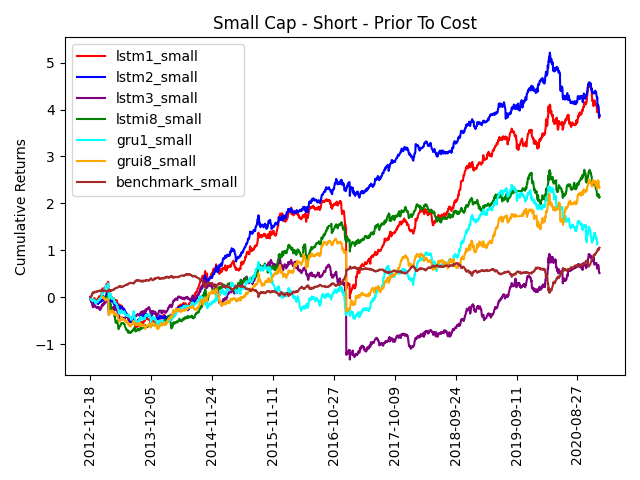
\includegraphics [scale=0.60,angle=360]{figures/cumulative_small_cap_return_no_cost_s.png}
\caption{Small cap trading performance short-only (K=5)}
\label{fig:shortsmall}
\end{figure} 
\indent\newline 
Comparing the networks with the benchmark shows each model being able to generate higher cumulative returns, except for the three-layered LSTM. However, when adjusting for risk, only the one- and two-layered LSTMs outperform the benchmark with higher Sharpe ratios.

\indent\newline 
\begin{table}[ht]
\centering
\resizebox{\textwidth}{!}{\begin{tabular}{l|cccccc|c}
\toprule
Annualized & \textbf{lstm1\_large} & \textbf{lstm2\_large} & \textbf{lstm3\_large} & \textbf{lstmi8\_large} & \textbf{gru1\_large} & \textbf{grui8\_large} & {\color[HTML]{656565} \textbf{benchmark\_large}} \\ \midrule
Return & -0.1142 & \textbf{-0.0300} & -0.0909 & -0.2030 & -0.1361 & -0.0946 & {\color[HTML]{656565} 0.1539} \\
Standard deviation & 0.2864 & 0.2730 & 0.2512 & 0.2786 & 0.2996 & \textbf{0.2429} & {\color[HTML]{656565} 0.1782} \\
Sharpe ratio & -0.4592 & \textbf{-0.1734} & -0.4308 & -0.7906 & -0.5121 & -0.4608 & {\color[HTML]{656565} 0.7670} \\
Max drawdown & 1.2328 & 0.8928 & 0.8715 & 1.6070 & 1.2907 & \textbf{0.8080} & {\color[HTML]{656565} 0.5535} \\
VaR 5\% & -0.5854 & \textbf{-0.4791} & -0.5043 & -0.6614 & -0.6289 & -0.4942 & {\color[HTML]{656565} -0.1391} \\ \bottomrule
\end{tabular}}
\caption{Large cap trading performance short-only (K=5)}
\end{table}
\indent\newline 
An analysis of the large cap models highlights lstm2\_large as the network with the least-worst performance results. The RNN generates negative annualized returns of 3\% and has a Sharpe ratio of -0.17. A closer look at table 5.20 shows that none of the large cap models are able to realize higher returns or Sharpe ratios than the benchmark.
 
\indent\newline 
\begin{figure}[H]
\centering
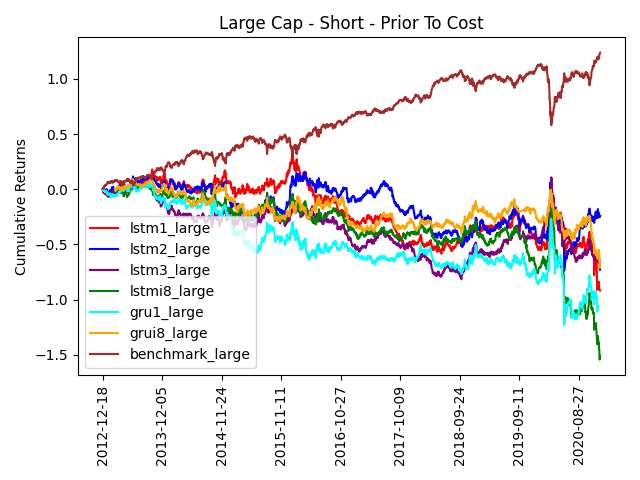
\includegraphics [scale=0.60,angle=360]{figures/cumulative_large_cap_return_no_cost_s.png}
\caption{Large cap trading performance short-only (K=5)}
\label{fig:shortlarge}
\end{figure} 
\indent\newline 
Similar to the small cap models the graph illustrates a negative correlation between the large cap RNNs and the benchmark. The reasoning behind this is that the trading strategy aims to capitalize on bearish market movements. This is especially visible during the market crash in 2020 with the break out of the Corona pandemic, where the benchmark returns drops with approximately 55 percentage points, while some of the RNNs' returns increase with approximately 40 percentage points.      
\indent\newline 
\begin{table}[ht]
\centering
\resizebox{\textwidth}{!}{\begin{tabular}{l|cc|c}
\toprule
Annualized & \textbf{lstm2\_small} & \textbf{lstm2\_large} & \textbf{Difference} \\ \midrule
Return & \textbf{0.4840} & -0.0300 & 0.5140 \\
Standard deviation & 0.4700 & \textbf{0.2730} & 0.1970 \\
Sharpe ratio & \textbf{0.9929} & -0.1734 & 1.1663 \\
Max drawdown & 1.3733 & \textbf{0.8928} & 0.4805 \\
VaR 5\% & \textbf{-0.2891} & -0.4791 & 0.1900 \\ \bottomrule
\end{tabular}}
\caption{Comparison of trading performance short-only (K=5)}
\end{table}
\indent\newline 
\begin{figure}[H]
\centering
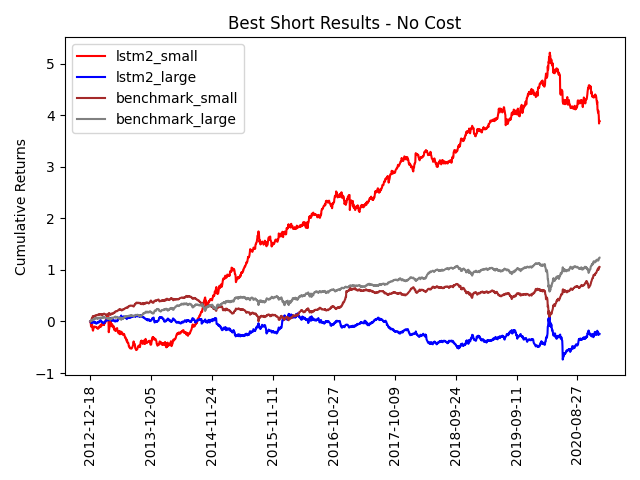
\includegraphics [scale=0.60,angle=360]{figures/cumulative_best_short_mix_return_no_cost.png}
\caption{Comparison of trading performance short-only (K=5)}
\label{fig:shortcomparison}
\end{figure} 
\indent\newline 
Assessing the best-performing model for each group of stocks prior to transaction costs shows how the small cap portfolio is able generate excess cumulative returns compared to the large cap portfolio and the benchmarks. The small cap portfolio has a 51 percentage points higher annualized return and a 1.16 higher Sharpe ratio than the large cap portfolio. The portfolio peaks during the market crash in 2020, where it capitalizes on the broad market fall. It seems the small cap model is able to profit from having the ability to learn patterns of a higher number of stocks within a long-term down trend and high volatility, compared to the large cap stocks that are more stable and have lower volatility.    

\subsection{Short-only after transaction costs}
This section presents an analysis on the short-portfolios where transaction costs are implemented for each trade. Lending rates for short-selling are not included in the backtesting. 
\indent\newline
\begin{table}[ht]
\centering
\resizebox{\textwidth}{!}{\begin{tabular}{l|cccccc|c}
\toprule
Annualized & \textbf{lstm1\_small} & \textbf{lstm2\_small} & \textbf{lstm3\_small} & \textbf{lstmi8\_small} & \textbf{gru1\_small} & \textbf{grui8\_small} & \textbf{benchmark\_small} \\ \midrule
Return & \textbf{-0.0944} & -0.1265 & -0.5823 & -0.2845 & -0.5210 & -0.3452 & 0.1313 \\
Standard deviation & 0.6705 & 0.4692 & 0.6186 & \textbf{0.4555} & 0.4747 & 0.6461 & 0.1773 \\
Sharpe ratio & \textbf{-0.1667} & -0.3065 & -0.9692 & -0.6625 & -1.1339 & -0.5611 & 0.6435 \\
Max drawdown & 2.4686 & \textbf{1.9144} & 4.6865 & 2.1632 & 4.3239 & 2.9465 & 0.3295 \\
VaR 5\% & -1.1973 & \textbf{-0.8983} & -1.6000 & -1.0339 & -1.3020 & -1.4080 & -0.1602 \\
Total number of trades & 13,193 & 14,011 & 14,835 & \textbf{12,151} & 15,231 & 14,031 & - \\ \bottomrule
\end{tabular}}
\caption{Small cap trading performance short-only w/t.cost (K=5)}
\end{table}
\indent\newline
Table 5.22 ranks lstm1\_small as the least-worst model when assessing annualized returns and returns adjusted for risk. It generates negative returns of 9.44\% and a negative Sharpe ratio of 0.16. Reviewing each model's performance suggest that the portfolio strategy does not show promising results, in light of none of the models being able to outperform the benchmark or generate positive returns.  
\indent\newline 
\begin{figure}[H]
\centering
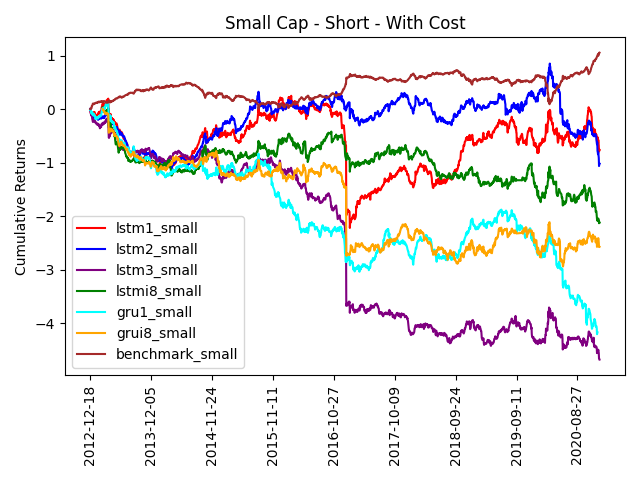
\includegraphics [scale=0.60,angle=360]{figures/cumulative_small_cap_return_with_cost_s.png}
\caption{Small cap trading performance short-only w/t.cost (K=5)}
\label{fig:shortlsmallc}
\end{figure} 
\indent\newline 
The lstm2\_small network outperforms the benchmark during a short period in 2020 (during the Corona market crash), but it experiences its highest drawdown right after, as the market quickly moves into another period characterized as a "bull-market". 

\indent\newline
\begin{table}[ht]
\centering
\resizebox{\textwidth}{!}{\begin{tabular}{l|cccccc|c}
\toprule
Annualized & \textbf{lstm1\_large} & \textbf{lstm2\_large} & \textbf{lstm3\_large} & \textbf{lstmi8\_large} & \textbf{gru1\_large} & \textbf{grui8\_large} & \textbf{benchmark\_large} \\ \midrule
Return & -0.7165 & \textbf{-0.6497} & -0.7351 & -0.7673 & -0.7779 & -0.7900 & 0.1539 \\
Standard deviation & 0.2855 & 0.2722 & 0.2509 & 0.2782 & 0.2989 & \textbf{0.2431} & 0.1782 \\
Sharpe ratio & -2.5699 & \textbf{-2.4498} & -2.9986 & -2.8201 & -2.6601 & -3.3205 & 0.7670 \\
Max drawdown & 5.7561 & \textbf{5.2951} & 5.9017 & 5.7403 & 6.2414 & 5.8861 & 0.0582 \\
VaR 5\% & -1.1862 & \textbf{-1.0975} & -1.1478 & -1.2250 & -1.2697 & -1.1900 & -0.1391 \\
Total number of trades & 13,821 & 14,219 & 14,781 & \textbf{12,001} & 14,669 & 14,789 & - \\ \bottomrule
\end{tabular}}
\caption{Large cap trading performance short-only w/t.cost (K=5)}
\end{table}
\indent\newline
The findings from analyzing the large cap models' performance when applied to a short-only portfolio shows extremely poor results. The different RNNs generate negative annualized returns between 60\% and 80\% and negative Sharpe ratios between 2.44 and 3.32. It would require regularly adding funds to the portfolios to be able to produce the results from the backtesting, as the models drop below 100\% in total cumulative returns.  
\indent\newline 
\begin{figure}[H]
\centering
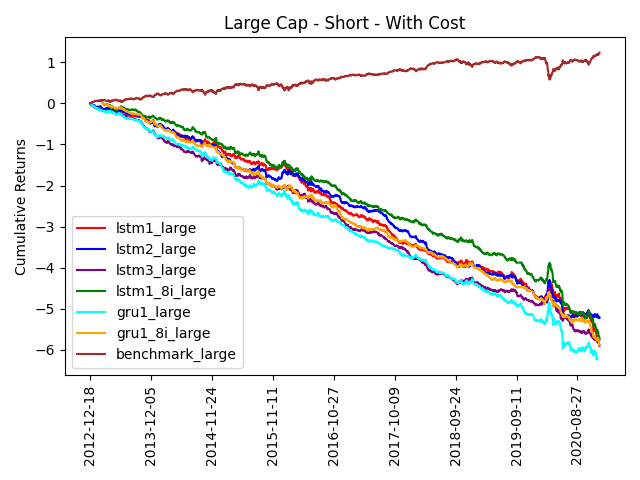
\includegraphics [scale=0.60,angle=360]{figures/cumulative_large_cap_return_with_cost_s.png}
\caption{Large cap trading performance short-only w/t.cost (K=5)}
\label{fig:shortlargec}
\end{figure} 
\indent\newline 
The figure above further illustrates the poor performance of the large cap models, where transaction costs increase the negative cumulative returns. The least-worst model (lstm2\_large) ends with cumulative returns of -521\%, while the worst model (gru1\_large) realizes cumulative returns of -622\%.

\indent\newline 
\begin{table}[ht]
\centering
\resizebox{\textwidth}{!}{\begin{tabular}{l|cc|c}
\toprule
Annualized & \textbf{lstm1\_small} & \textbf{lstm2\_large} & \textbf{Difference} \\ \midrule
Return & \textbf{-0.0944} & -0.6497 & 0.5553 \\
Standard deviation & 0.6705 & \textbf{0.2722} & 0.3983 \\
Sharpe ratio & \textbf{-0.1667} & -2.4498 & 2.2831 \\
Max drawdown & \textbf{2.4686} & 5.2951 & -2.8265 \\
VaR 5\% & \textbf{-1.1973} & -1.0975 & -0.0998 \\
Total number of trades & \textbf{13,193} & 14,219 & -1,026 \\ \bottomrule
\end{tabular}}
\caption{Comparison of trading performance short-only w/t.cost (K=5)}
\end{table}
\indent\newline 
\begin{figure}[H]
\centering
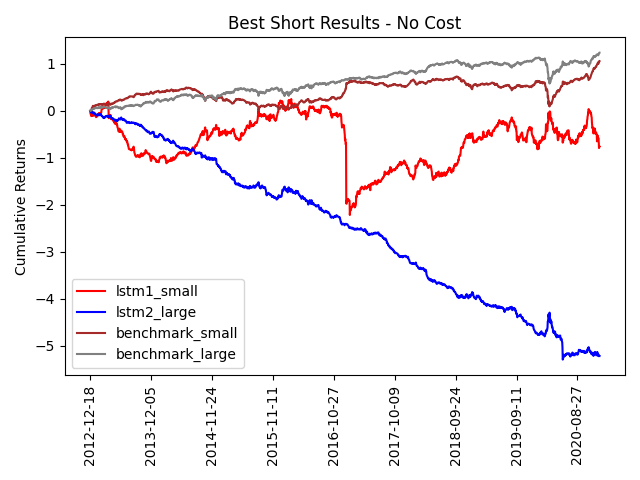
\includegraphics [scale=0.60,angle=360]{figures/cumulative_best_short_mix_return_cost.png}
\caption{Comparison of trading performance short-only w/t.cost (K=5)}
\label{fig:shortcomparisonc}
\end{figure} 
\indent\newline 
Analyzing the top-performing model for both small cap and large cap stocks after including transaction costs, reveals that the RNNs should not be employed to short-only portfolios. While neither model is able to generate positive returns, there are still significant differences in portfolio performance. The lstm1\_small generates a 55 percentage points higher annualized return and a 2.28 higher Sharpe ratio, which translates into a difference in cumulative returns of 445 percentage points. Choosing a portfolio strategy consisting of only shorting stocks, where positions are opened and closed on a daily basis, may not be a realistic trading strategy. This is because short-selling requires lending shares, which may not be available at all times or for all stocks. 

\section{Summary of Results}
The resulting findings suggest RNNs can be employed to predicting small cap stock returns for all portfolio strategies and outperform large cap stocks and relevant benchmarks, except short-only (after accounting for transaction costs). The lstm1\_small network is the most suitable model for predicting small cap stock returns, and generates the overall best portfolio results. Providing the models with extra input features do not seem to improve model performance, which can be a result of the main input feature of previous returns reflecting the impact of all the additional independent variables. An overall risk assessment finds the small cap model to have less downside risk. The large cap models show inferior performance in terms of max drawdown and value at risk. The list below summarize the difference in annualized Sharpe ratio for the top-performing small cap and large cap models for each portfolio strategy.

\indent\newline
\textbf{Annualized Sharpe ratio prior to transaction costs:}
\indent\newline
\textbf{Long portfolio} 
\indent\newline
lstm1\_small: \underline{3.17},  grui8\_large: \underline{0.84},  Difference: \underline{2.33}

\indent\newline
\textbf{Long-short portfolio} 
\indent\newline
lstm1\_small: \underline{2.67},  lstm2\_large: \underline{0.50},  Difference:  \underline{2.17}  

\indent\newline
\textbf{Short portfolio} 
\indent\newline
lstm2\_small: \underline{0.99},  lstm2\_large: \underline{-0.17},  Difference: \underline{1.16} 

\indent\newline
\indent\newline
\textbf{Annualized Sharpe ratio after transaction costs:}
\indent\newline
\textbf{Long portfolio} 
\indent\newline
lstm1\_small: \underline{1.92},  lstmi8\_large: \underline{-1.62},  Difference: \underline{3.54}

\indent\newline
\textbf{Long-short portfolio}
\indent\newline
lstm1\_small: \underline{2.17},  lstm2\_large: \underline{-0.93},  Difference: \underline{3.10} 
  
\indent\newline
\textbf{Short portfolio} 
\indent\newline
lstm1\_small: \underline{-0.16},  lstm2\_large: \underline{-2.45},  Difference: \underline{2.29}  